\chapter{Recent changes to the vacuum system} \label{app:breakingVacuum}
In the following sections, we give some reference data for when the vacuum system was open at the end of 2017.
The thermocouple measurements and such are printouts from the OneNote section "Vacuum chamber".

\section{Nozzle redesign - nuiNozzle 2018}
During the downtime from breaking vacuum, we attempted to redesign our atom nozzle to include a heat shield. A CAD image is shown in figure. Unfortunately, due to the high tolerances of the base flange and surrounding enclosure the machining required for this custom piece was deemed prohibitively expensive. A prototype was designed following the machine drawings available in \texttt{Drobo:\textbackslash Neutral\textbackslash Laboratory Systems\textbackslash Vacuum Chamber\textbackslash 2017 - Nozzle Redesign - NUI nozzle} but was abandoned due to a bend that developed in the tubing which holds the fire rod. 

In addition to the heat shield, we also attempted to incorporate a design feature from Plasma's nozzle redesign which addressed the fragility of the feedthrough connection to the heater wire. 
This was a problem because the heater wire connection is very thin and we used large clamp type connection for them before which was problematic due to the fragility of the heater wire and the necessity that the bulky clamp couldn't touch the nozzle body (as this would short the heater connection). 
The new connection would allow us to use a smaller crimp to the heater wire, use the rigidity of the feedthrough itself, and use alumina screws to insulate the connection from the nozzle body.
	
	\begin{figure} 
		\centerline{
		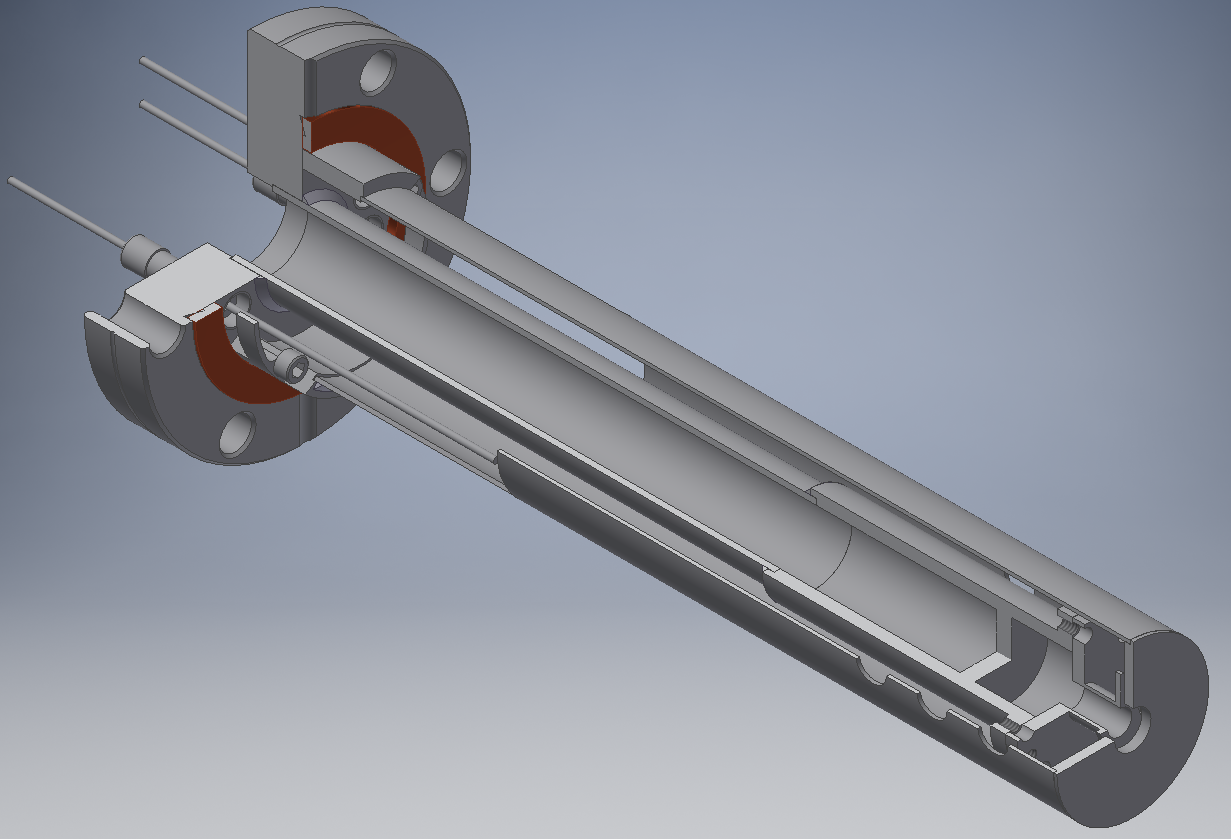
\includegraphics[width=\textwidth]{neuNozzle_partial.png}}
		\caption{Redesigned neutral strontium oven, nuiNozzle}{}
		\label{fig:nuiNozzle}
	\end{figure}

Finally, I had some trouble finding the part number associated with the firerod in the Neutral chamber but luckily I found one of the broken firerods still had it's part number on it, SK7J-2953. 
Below is the info from Valin Corporation who seems to be the local reseller of Watlow products.

\begin{verbatim}
SPECIAL DIAMETER
HT FIREROD   
T/C CENTER CORE LOC “A” TYPE “J”
 
120 Volts
240 watts
0.580 +/- 0.004 Diameter firerod
7.5” length
12” of MGT leads
12” of TC leads
6 13/32” of no heat section at lead end.
Crimped of leads construction.
\end{verbatim}

\section{Opening vacuum - data and setup}
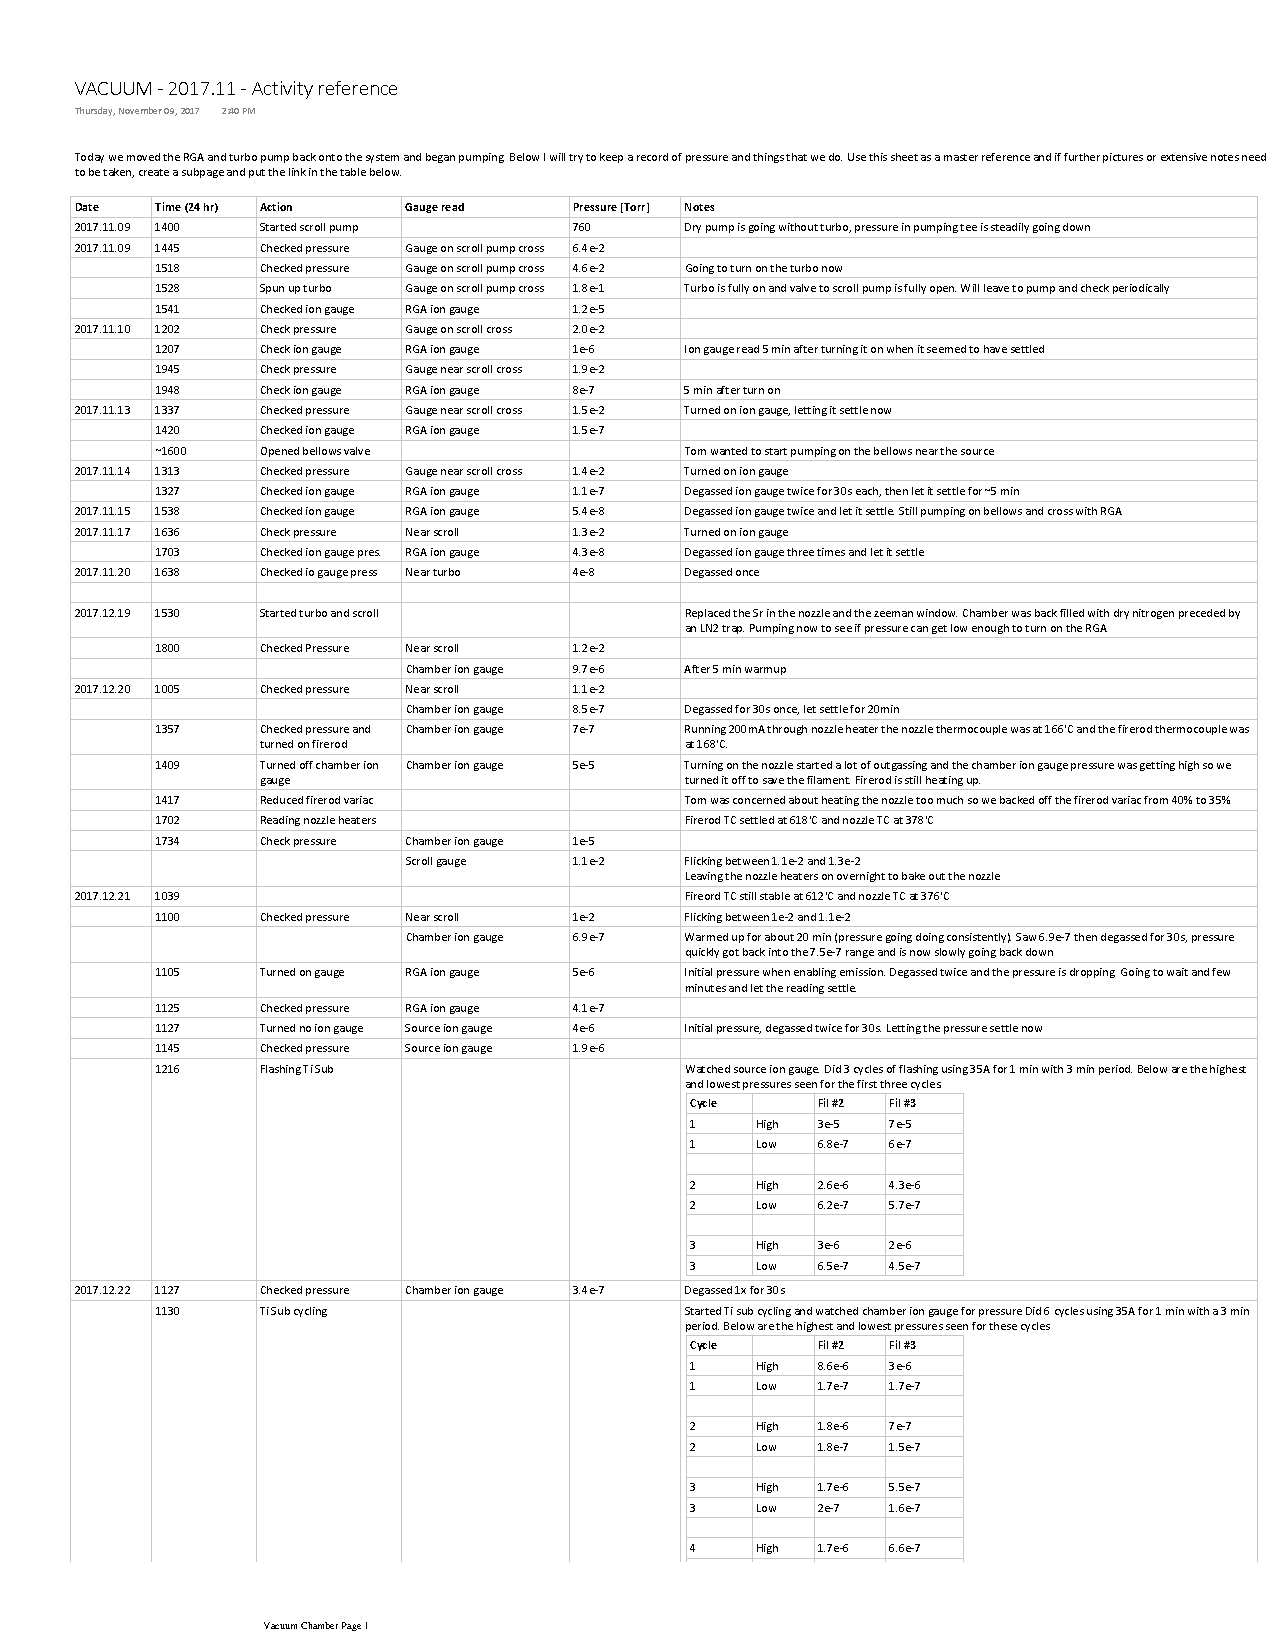
\includepdf[pages=-]{VacuumChamber.pdf}
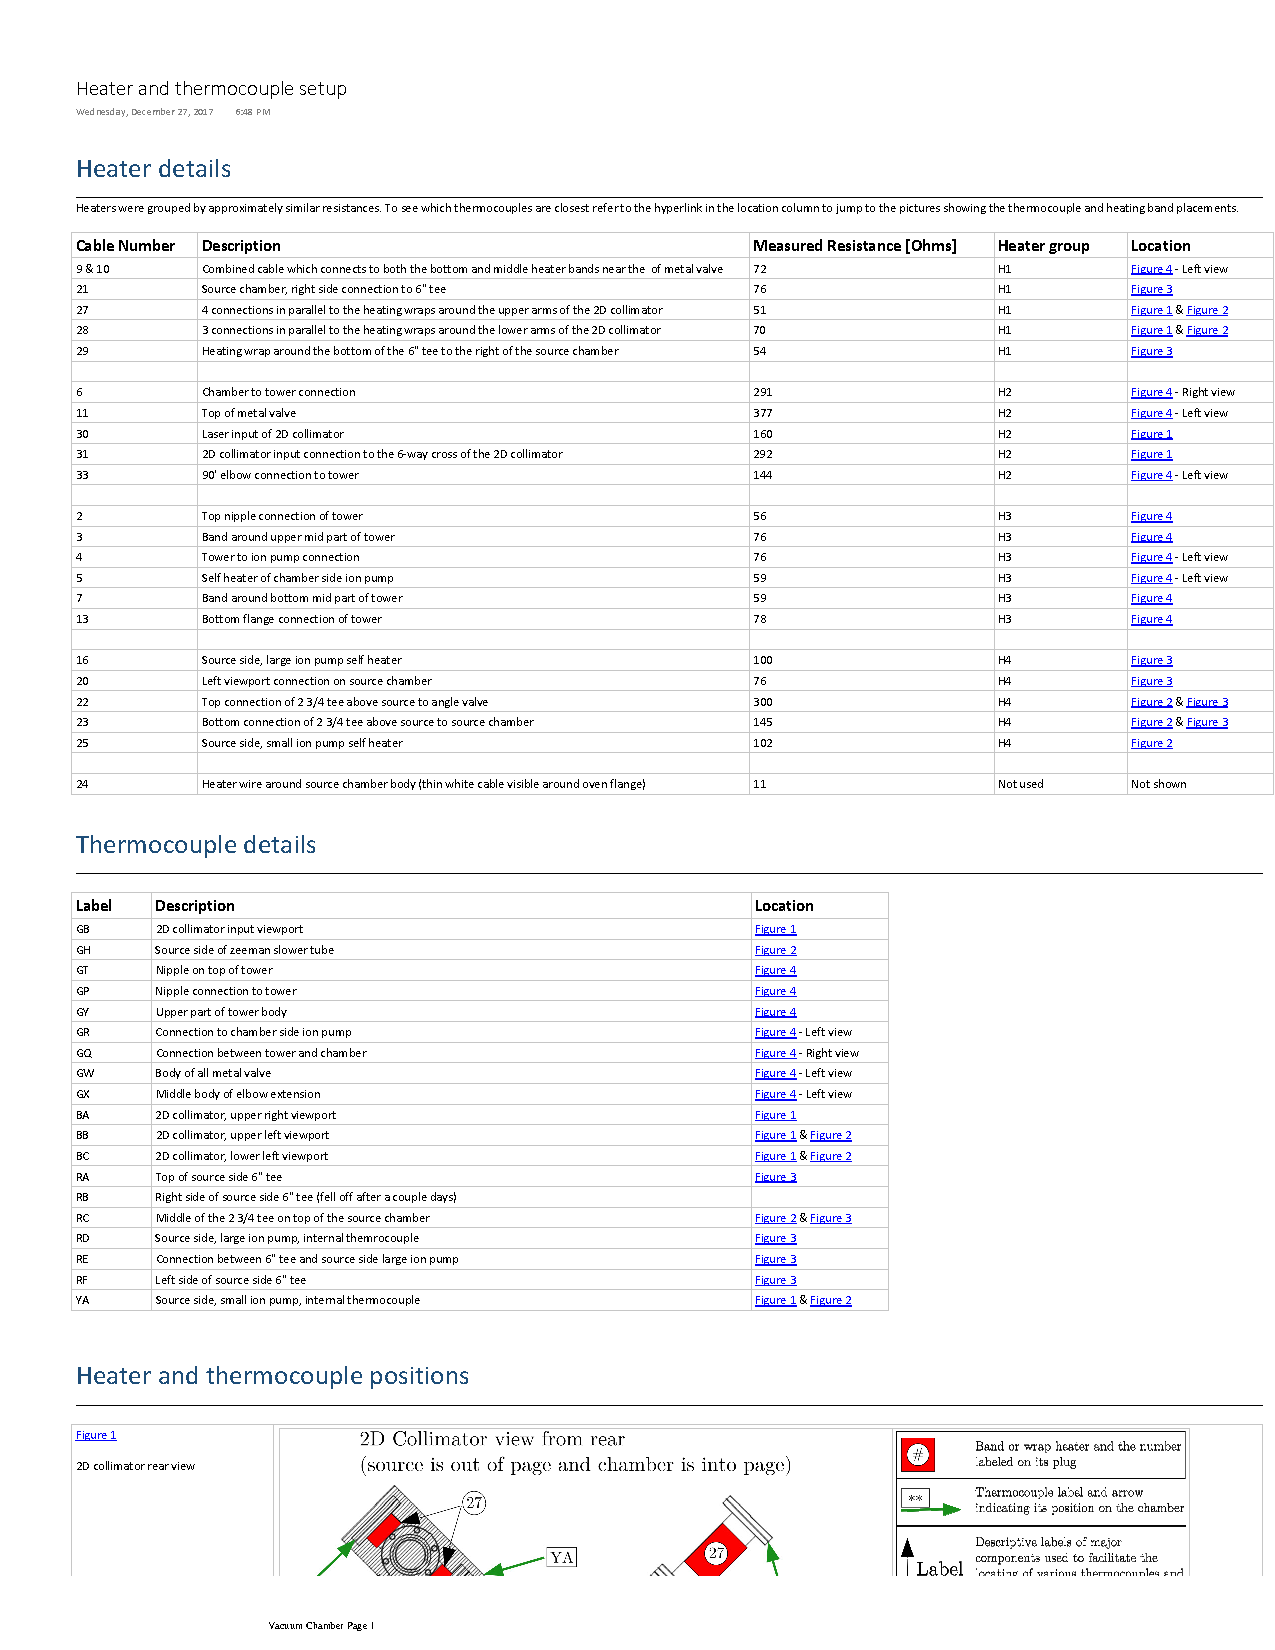
\includepdf[pages=-]{thermocoupleSetup.pdf}
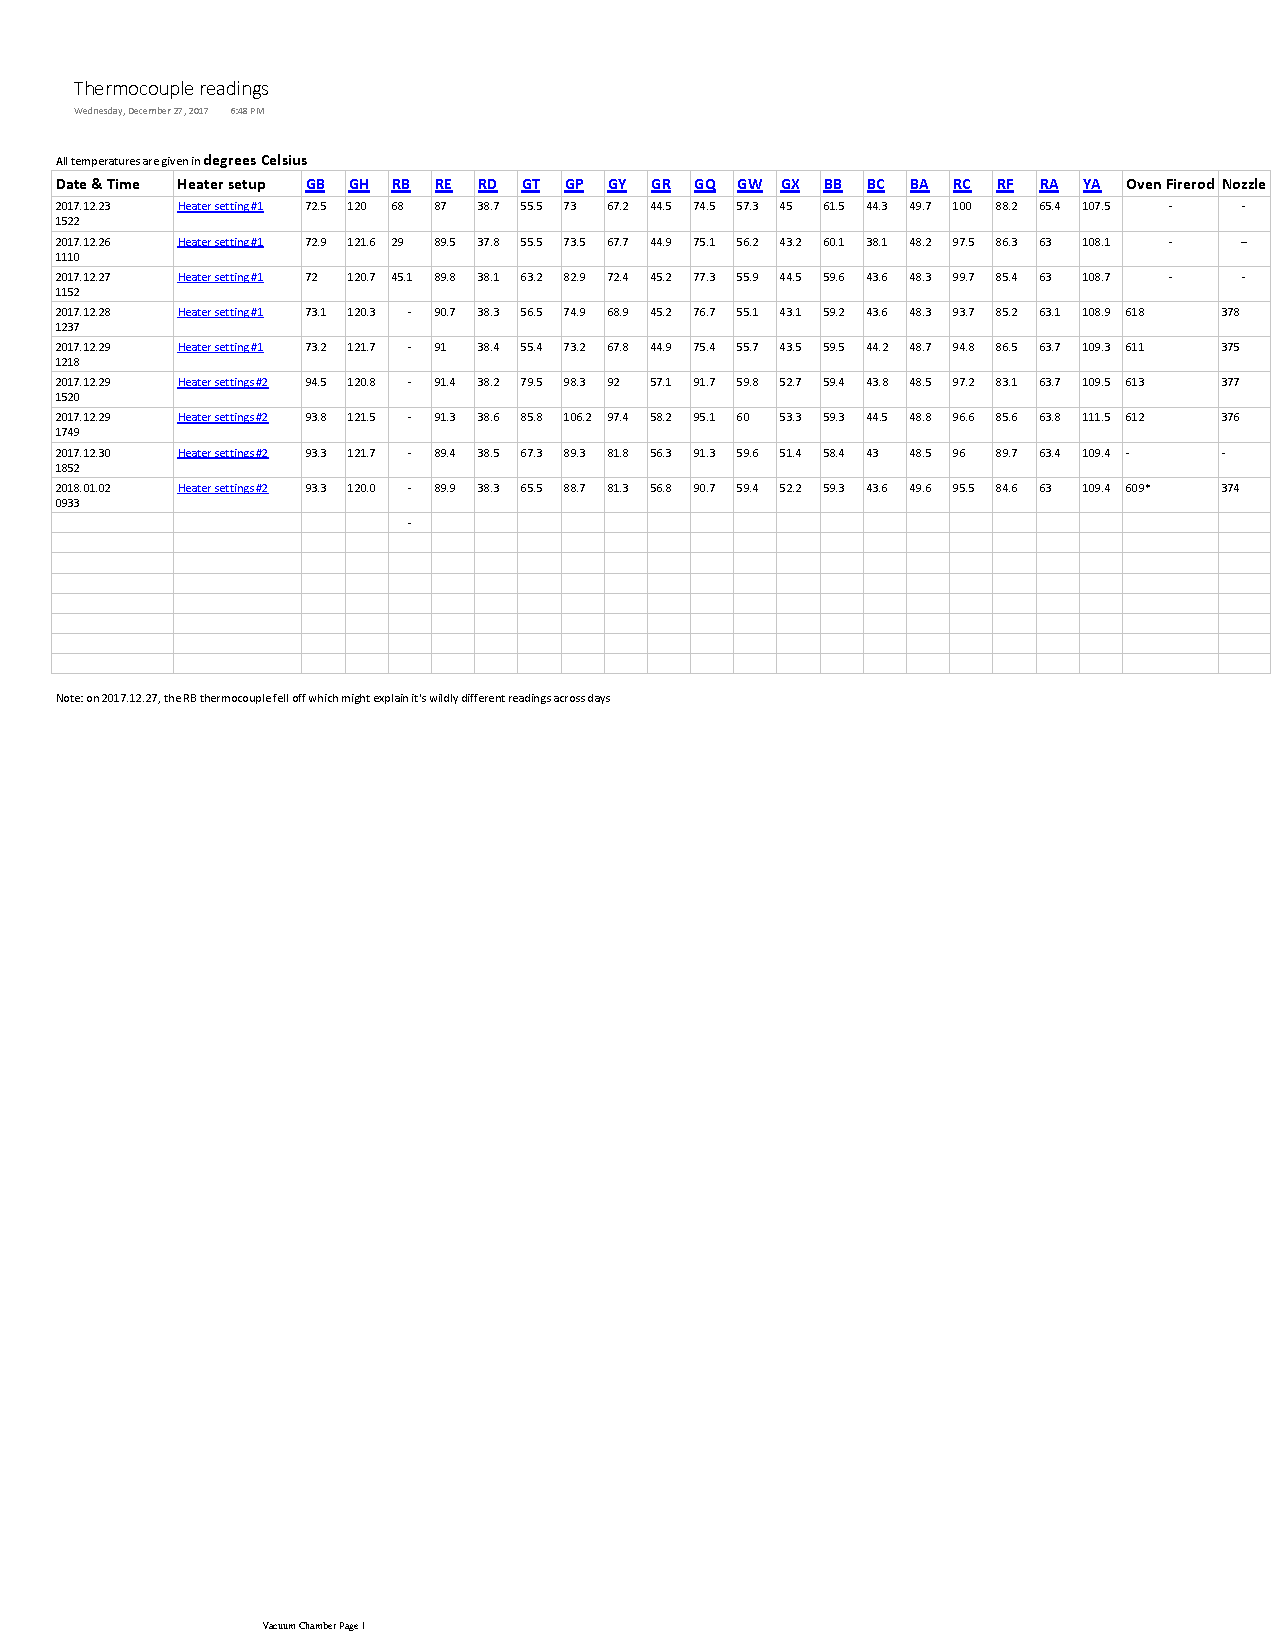
\includepdf[pages=-]{thermocoupleReadings.pdf}
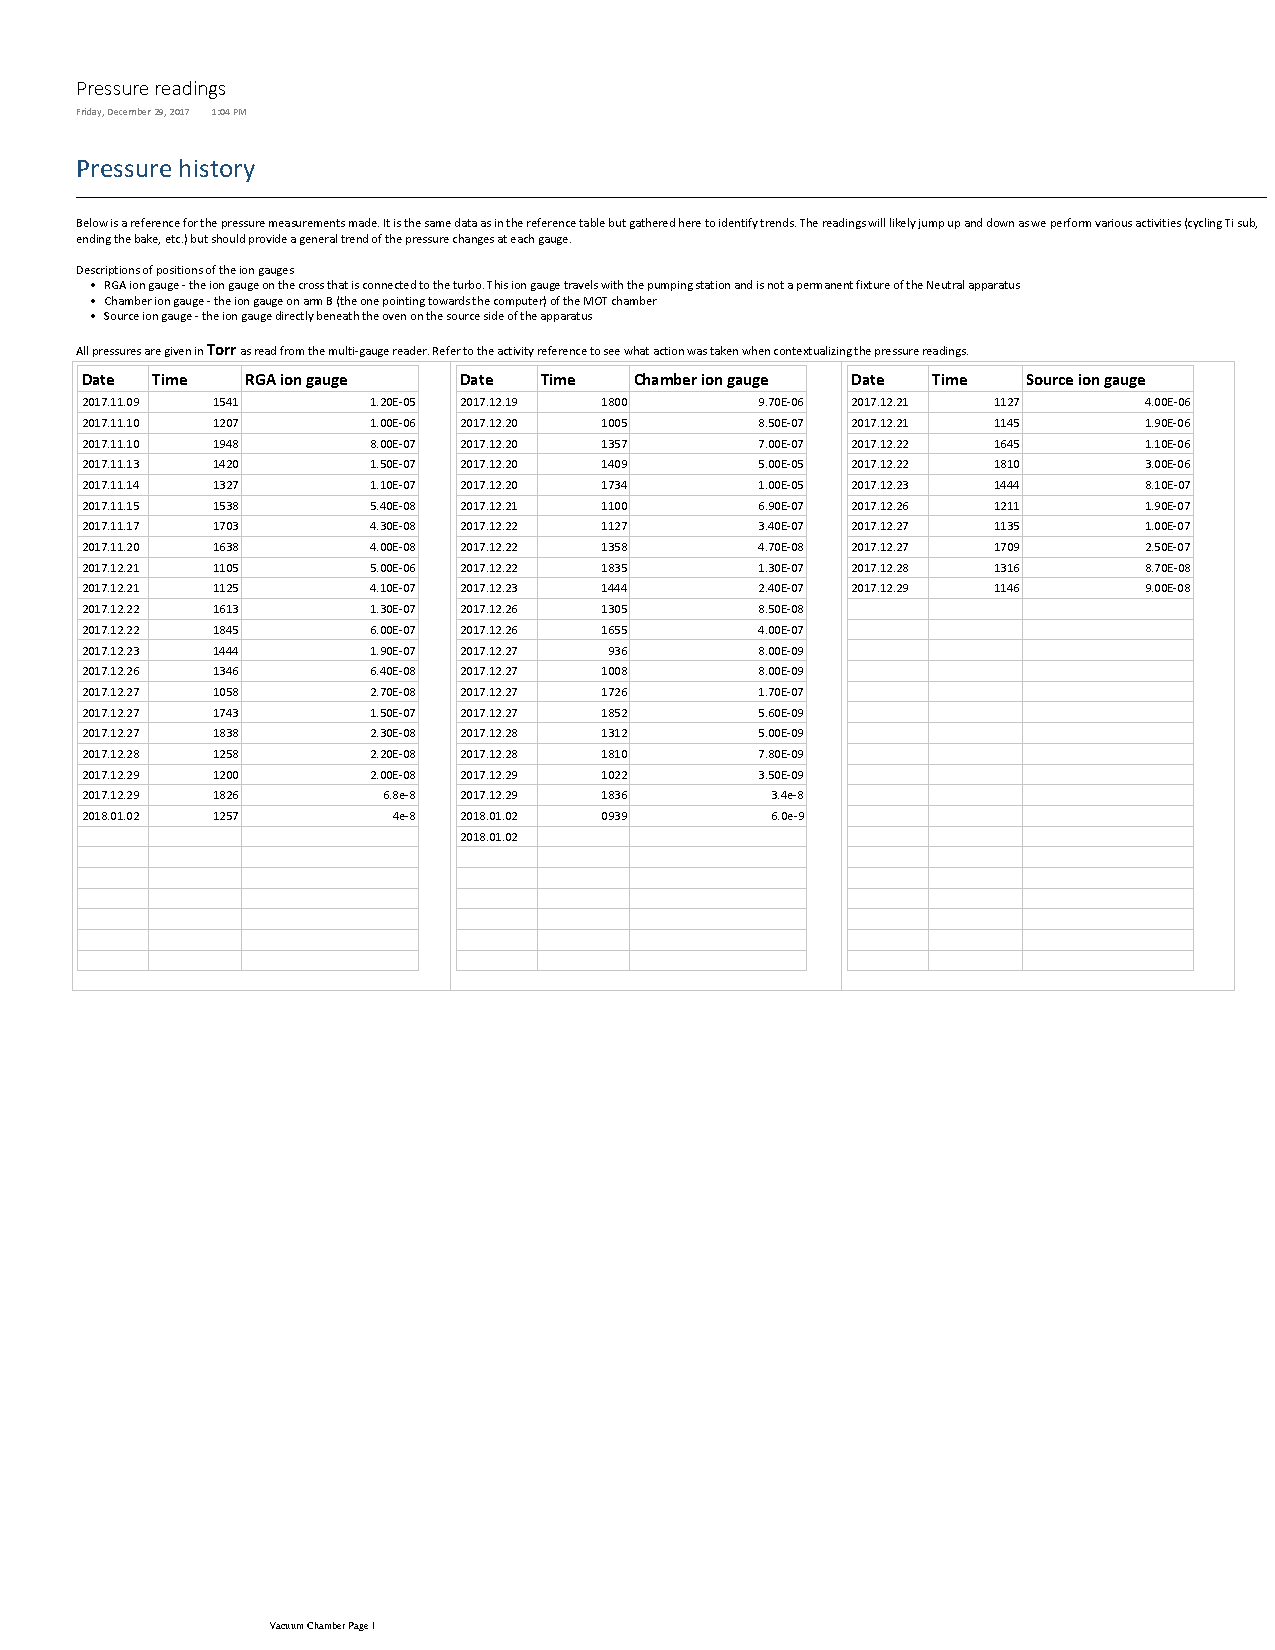
\includepdf[pages=-]{pressureHistory.pdf}
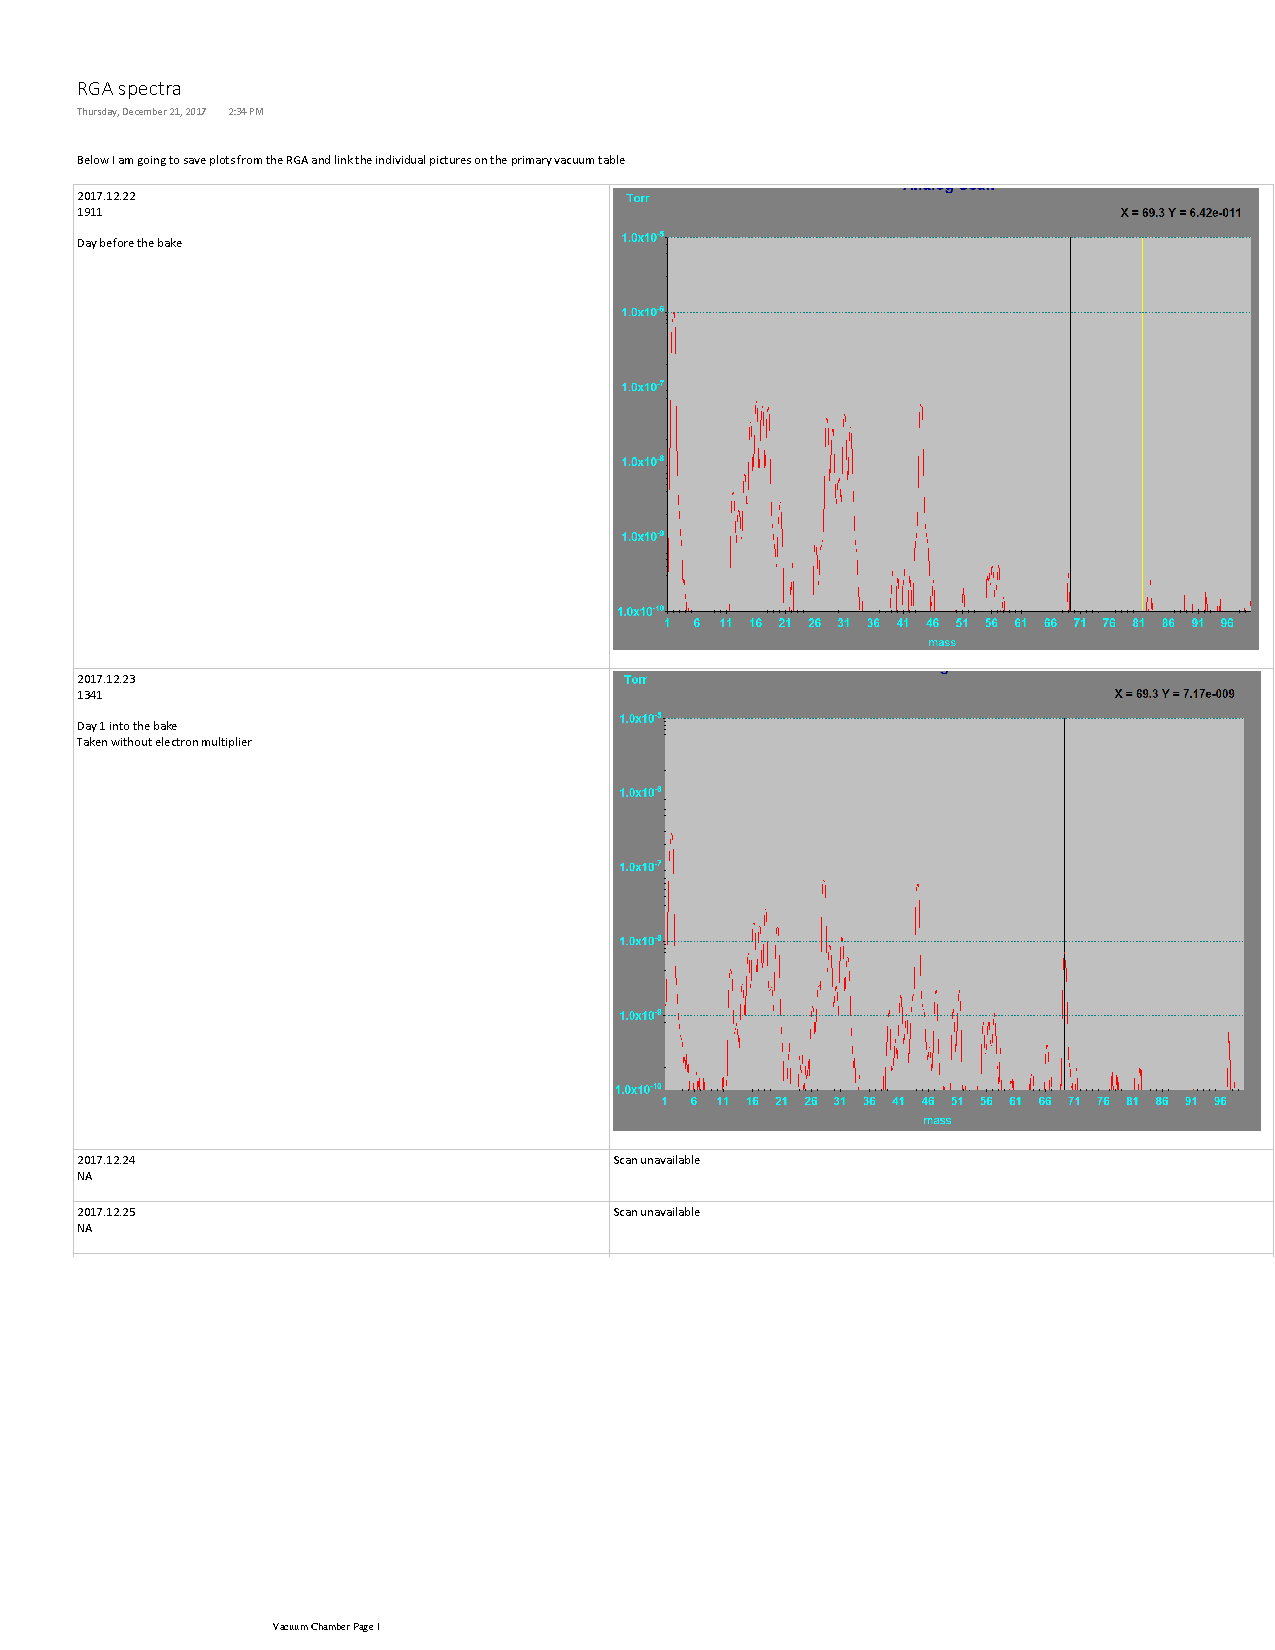
\includepdf[pages=-]{RGASpectra.pdf}

%%%%%%%%
%Z:\Neutral\Laboratory Systems\Vacuum Chamber\2017 - Nozzle Redesign - NUI nozzle

%We hypothesized that lack of a heat shield led to uneven distribution of the thermal energy throughout the oven.
%Therefore, fastening of the heat shield to the base flange was the primary goal of the redesign undertaken in late 2017 and further details can be found in App. \ref{app:breakingVacuum}. 
%
% we did not install the gate valve before re-establishing vacuum. 
%
%The hope in doing this upgrade was to provide a better method for replacing the end cap window which the atom source directly points at. 
%
%With that fun aside, we oder an extra window and the gate valve to replicate the system put in place on the Rydberg appartus so that future needs to repalce the window coul be accomplished by simply back filling the chamber with dry nitrogen or argon, closing the gate valve and simply replacing it quickly without the need to expose the main chamber body to direct atmospheric gas. 
%
%
%
%However, the largest constraint was due to the flange size of 2 3/8" as the basis for the design. This provides very tight confinement and w
%
%What is the model number for the firerod? What were the materials that were used? 

%%%%%

%Don't forget the plan was 
%
%Other reason for redesign was to attach the heat shield directly to the flange.
%
%All the pieces were ordered and built but a mistake on turning the nozzle body meant that we couldn't use the nozzle we built. As of April 2019, this construction is located in \hl{somewhere}